%\title{LaTeX Portrait Poster Template}
%%%%%%%%%%%%%%%%%%%%%%%%%%%%%%%%%%%%%%%%%
% a0poster Portrait Poster
% LaTeX Template
% Version 1.0 (22/06/13)
%
% The a0poster class was created by:
% Gerlinde Kettl and Matthias Weiser (tex@kettl.de)
% 
% Adapter by Jens Buysse for Hogeschool Gent
% This template has been downloaded from:
% http://www.LaTeXTemplates.com
%
% License:
% CC BY-NC-SA 3.0 (http://creativecommons.org/licenses/by-nc-sa/3.0/)
%
%%%%%%%%%%%%%%%%%%%%%%%%%%%%%%%%%%%%%%%%%

%----------------------------------------------------------------------------------------
%	PACKAGES AND OTHER DOCUMENT CONFIGURATIONS
%----------------------------------------------------------------------------------------

\documentclass[a0,portrait]{a0poster}

\usepackage{multicol} % This is so we can have multiple columns of text side-by-side
\columnsep=100pt % This is the amount of white space between the columns in the poster
\columnseprule=3pt % This is the thickness of the black line between the columns in the poster

\usepackage[svgnames]{xcolor} % Specify colors by their 'svgnames', for a full list of all colors available see here: http://www.latextemplates.com/svgnames-colors

\usepackage{times} % Use the times font
%\usepackage{palatino} % Uncomment to use the Palatino font

\usepackage{graphicx} % Required for including images
\graphicspath{{figures/}} % Location of the graphics files
\usepackage{booktabs} % Top and bottom rules for table
\usepackage[font=small,labelfont=bf]{caption} % Required for specifying captions to tables and figures
\usepackage{amsfonts, amsmath, amsthm, amssymb} % For math fonts, symbols and environments
\usepackage{wrapfig} % Allows wrapping text around tables and figures
\usepackage[export]{adjustbox}
\usepackage{tabularx}

\begin{document}

%----------------------------------------------------------------------------------------
%	POSTER HEADER 
%----------------------------------------------------------------------------------------

% The header is divided into two boxes:
% The first is 75% wide and houses the title, subtitle, names, university/organization and contact information
% The second is 25% wide and houses a logo for your university/organization or a photo of you
% The widths of these boxes can be easily edited to accommodate your content as you see fit

\begin{minipage}[t]{0.75\linewidth}
\VeryHuge \color{HoGentAccent1} \textbf{Kan de PWA de native applicatie vervangen ?} \color{Black}\\ % Title
\huge \textbf{Verdurme Robbie, Delrue bart, Smits Lieven}\\[0.5cm] % Author(s)
\huge Hogeschool Gent, Valentin Vaerwyckweg 1, 9000 Gent\\[0.4cm] % University/organization
\Large \texttt{robbie.verdurme@hogent.be} \\
\end{minipage}
%
\begin{minipage}[t]{0.25\linewidth}

\includegraphics[width=13cm,right]{figures/HOGENT_Logo_Pos_rgb.png} 

\end{minipage}

\vspace{1cm} % A bit of extra whitespace between the header and poster content

%----------------------------------------------------------------------------------------

\begin{multicols}{2} % This is how many columns your poster will be broken into, a portrait poster is generally split into 2 columns

%----------------------------------------------------------------------------------------
%	ABSTRACT
%----------------------------------------------------------------------------------------

\color{HoGentAccent1} % Navy color for the abstract

\begin{abstract}
In dit onderzoek werd nagegaan in welke mate de progressive web applicatie de native applicatie kan vervangen. Om dit te testen werd er een zelfde applicatie gemaakt zowel in progressive web applicatie vorm als in native applicatie vorm. Eens deze applicaties klaar waren, werden deze getest op vlak van snelheid, gebruiksvriendelijkheid en de benodigde ruimte die de applicatie inneemt op het apparaat. Uit het onderzoek bleek dat de progressive web applicatie 90.67\% kleiner is dan de native applicatie maar niet sneller is. De native applicatie had een gemiddelde van 2.360 seconden terwijl de progressive web applicatie een gemiddelde van 2.693 seconden behaalde op het filteren van een menu.
\end{abstract}
%----------------------------------------------------------------------------------------
%	INTRODUCTION
%----------------------------------------------------------------------------------------

\color{HoGentAccent1} 
\section*{Introductie}
\color{black}
\color{black}
De native applicatie kent al een aantal jaren succes op de markt, dit is ondermeer te danken aan de komst van de play- en app store. Maar niet iedereen heeft toegang tot dit platform, denk aan huawei die met zijn eigen store op de markt komt. De applicaties die op een store platform beschikbaar zijn, zijn meestal wel een aantal megabyte groot en  dit is een probleem voor mensen die weinig ruimte hebben op hun apparaat. Een oplossing hiervoor is de progressive web applicatie. Een progressive web applicatie is een webapplicatie die offline beschikbaar kan gemaakt worden voor de gebruiker. Indien de gebruiker dat wenst kan deze als applicatie geïnstalleerd worden op het apparaat om het gevoel van een native applicatie na te bootsen. Om deze reden komen we tot de volgende onderzoeksvraag,  kan de PWA de native applicatie vervangen?
%----------------------------------------------------------------------------------------
%	GEOLOGY
%----------------------------------------------------------------------------------------

\color{Black} % DarkSlateGray color for the rest of the content
\color{HoGentAccent1} 
\section*{Experimenten}
\color{black}
Om na te gaan of de progressive web applicatie de native applicatie zou kunnen vervagen, werden er twee testen uitgevoerd op vlak van snelheid, gebruiksvriendelijkheid en werd de benodigde plaats vergeleken van de applicaties.

Een van de testen die werd uitgevoerd op beide applicaties is het opvragen en navigeren naar de detailpagina van een menu. Onderstaande grafiek geeft de resultaten hiervan weer.

\begin{center}
	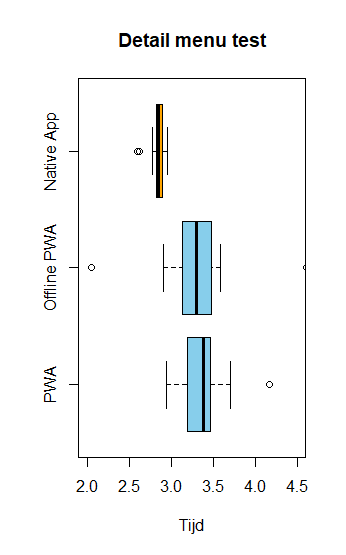
\includegraphics[width=200px]{Rplot_DetailMenu_AllType}
	\captionof{figure}{\color{HoGentAccent5} Detail menu ophalen test}
\end{center}

\begin{center}
		\centering
	\begin{tabular}{|c|c|c|c|c|c|}
		\hline
		Type        & Min.  & 1ste Qu. & Gemiddelde & 3de Qu. & Max.  \\
		\hline
		PWA         & 2.940 & 3.205    & 3.380      & 3.465   & 4.170 \\
		\hline
		Offline PWA & 2.050 & 3.138    & 3.292      & 3.478   & 4.610 \\
		\hline
		Native App  & 2.596 & 2.826    & 2.846      & 2.901   & 2.952 \\
		\hline
	\end{tabular}
\end{center}

De andere test die werd uitgevoerd op beide applicaties is het opzoeken van een menu aan de hand van de filter.
\begin{center}
	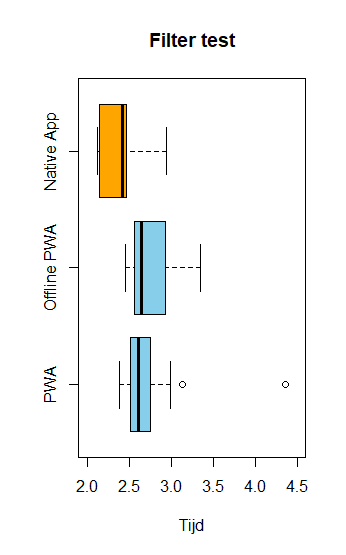
\includegraphics[width=200px]{Rplot_Filter_AllType}
	\captionof{figure}{\color{HoGentAccent5} Menu filteren test}
\end{center}

\begin{center}
		\centering
	\begin{tabular}{|c|c|c|c|c|c|}
		\hline
		Type        & Min.  & 1ste Qu. & Gemiddelde & 3de Qu. & Max.  \\
		\hline
		PWA         & 2.380 & 2.522    & 2.693      & 2.745   & 4.360 \\
		\hline
		Offline PWA & 2.460 & 2.565    & 2.752      & 2.992   & 3.350 \\
		\hline
		Native App  & 2.118 & 2.152    & 2.360      & 2.474   & 2.950 \\
		\hline
	\end{tabular}
\end{center}

Om de benodigde plaats te vergelijken, wordt er bekeken hoe groot de applicatie is van zodra de applicatie werd gedownload en eens de data werd opgevraagd. Er werd hiervoor gekozen omdat dat de progressive web applicatie zijn data offline cached en hierdoor meer ruimte zal innemen op het apparaat. 
\begin{center}
	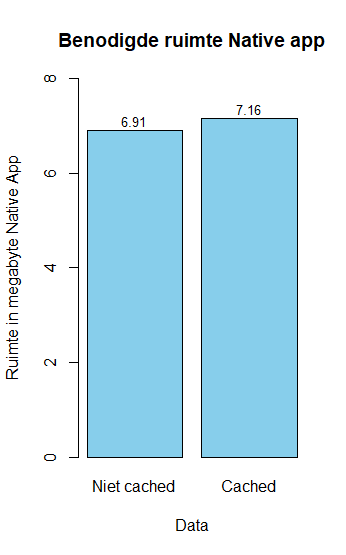
\includegraphics[width=200px]{Rplot_BenodigdeRuimte_NativeApp}
	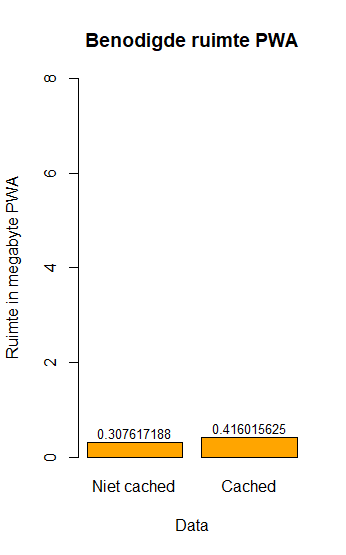
\includegraphics[width=200px]{Rplot_BenodigdeRuimte_PWA}
	\captionof{figure}{\color{HoGentAccent5} Benodigde ruimte applicaties}
\end{center}

\begin{center}
	\centering
\begin{tabular}{|c|c|c|}
	\hline
	Type              & Niet gecached    & Gecached    \\
	\hline
	PWA               & 0.307619188      & 0.416015625 \\
	\hline
	Native applicatie & 6.91             & 7.16        \\
	\hline
\end{tabular}
\end{center}

% TABLE

Om de gebruiksvriendelijkheid te testen werd gevraagd aan een aantal proefpersonen om een paar specifieke taken uit te voeren. Een van deze taken is het opzoeken van een menu met behulp van de filter. Dit was voor de meeste mensen geen probleem op de native applicatie. Bij de progressive web applicatie sprong de filter niet in het oog waardoor de proefpersonen meer moeite hadden om de taak uit te voeren. De tweede taak was het toevoegen van een menu. Dit bleek geen probleem te zijn voor de proefpersonen bij de beide applicaties. 

%------------------------------------------------



\color{HoGentAccent1} 
\section*{Conclusies}
\color{black}
Het doel van dit onderzoek was nagaan of de progressive web applicatie de native applicatie kan vervangen. Dit met behulp van twee identieke applicaties die getest werden op vlak van snelheid, gebruiksvriendelijkheid en de benodigde ruimte.

Uit de resultaten is gebleken dat de PWA even gebruiksvriendelijk is als de native applicatie maar dat deze tot 94.19\% of 6.74 Megabyte kleiner is. Helaas is dit niet voldoende om de native applicatie te kunnen vervangen. De PWA heeft nog geen toegang tot meer specifieke functionaliteiten zoals de bluetooth module, geofencing en communicatie met andere applicaties. Dit limiteert de PWA in functionaliteit ten opzichte van de native applicatie. Ten opzichte van de gebruiksvriendelijkheid en terugvindbaarheid heeft de native applicatie een groot voordeel vanwege de store waarin alle applicaties kunnen teruggevonden worden, hiervoor werd een oplossing gevonden voor de PWA maar dit heeft nog niet de goede ondersteuning.
Eens deze functionaliteiten toegevoegd zijn en de app store en play store een goede ondersteuning bieden voor een PWA zal dit een waardig alternatief zijn voor de native app.

%----------------------------------------------------------------------------------------
%	FORTHCOMING RESEARCH
%----------------------------------------------------------------------------------------
\color{HoGentAccent1} 
\section*{Toekomstig onderzoek}
\color{black}
De resultaten van de snelheidstesten werden behaald met een stabiele internetverbinding. Verder onderzoek is nodig om te bevestigen dat de progressive web applicatie trager is indien er geen netwerk verbinding is.
%----------------------------------------------------------------------------------------

\end{multicols}
\end{document}